\documentclass[]{article}
\usepackage[a4paper, margin=0.5in]{geometry}
\usepackage{graphicx}


%opening
\title{Solution for Problem Set D}
\author{
	Beshoy Saad, 2572741\\
	Rutuja Saptarshi, 2572864\\
	Vage Mkrtchyan, 2567128
}

\begin{document}

\maketitle

\section{Problem D1: Hardware Redundancy}
\begin{itemize}
	\item[a] Hardware redundancy:
	\begin{itemize}
			\item[i]Static Hardware redundancy is based on voting. It uses the concept of fault masking and consists of a voter that forwards the majority vote of all inputs.
		\begin{figure}[h]
			\centering
			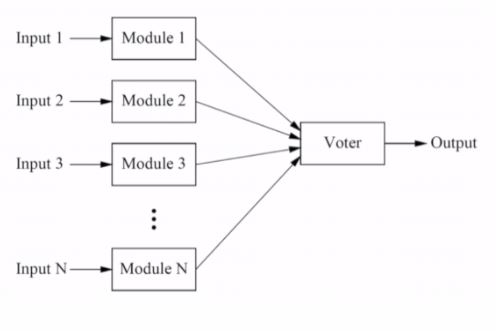
\includegraphics{Static}  
			\caption{Static hardware redundancy}
		\end{figure}
		
		
		Reliability of the voter is high because of low complexity.
		\item[ii] Dynamic hardware redundancy : Output of the module at any instance is determibed by only one module. Fault Detector is used in dymanic hardware redundancy which observes input and activates output of other module ("spare") if error observed.
		\begin{figure}[h]
			\centering
			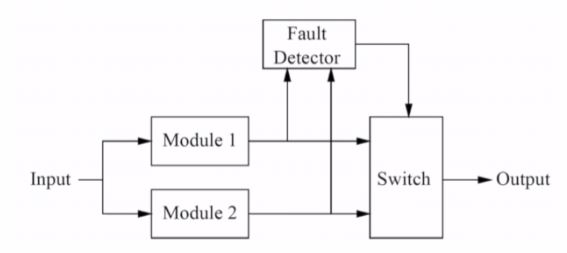
\includegraphics{Dynamic}  
			\caption{Dynamic hardware redundancy}
		\end{figure}
	\end{itemize}

	\item[b] Setup chosen for each application
	\begin{itemize}
			\item[i]Dynamic hardware redundancy setup with two modules and one fault detector.\\Justification:Module is 98\% reliable upto 1 year. Hence chances of it's failure are very low. Module is used in mission only for 30mins after which it is replaced.In case one module fails  during the flight, fault is detected by the fault detector and output is switched to other module. Using static setup with 3 modules and one voter will lead to excess expenditure(since module costs significant amout of money) and size. Hence using dynamic hardware redundancy in this application is cost effective and also reliable.
		\item[ii]Static hardware redundancy setup with three modules and one voter.\\Justification:Module is 99.5\% reliable upto only 1 year whereas it is used in an application for 50 years. There are chances of the module becoming faulty after a period of time. Using 3 modules and a voter helps in masking the fault of one module. Also, since module is a part of a satellite, replacement of module if it becomes faulty is very difficult. Thus, taking into consideration the duraion of usage and difficulty of replacement of module, it is better to take majority vote out of the 3 modules. Hence static hardware redundancy is preferable.
		\item[iii]Dynamic hardware redundancy setup with two modules and one fault detector.\\Justification:Module is 99\% reliable upto 1 year and is used in an applicaiton which is not very critical. Also, it is checked for failures once a day when it may or may not be replace. If a module is faulty, fault detector will detect the fault and switch the output to other module. The faulty module can then be replaced during daily checking.  Using static setup with 3 modules and one voter will lead to excess expenditure(since module costs significant amout of money) and size.  Hence using dynamic hardware redundancy in this application is best solution.
	\end{itemize}

\end{itemize} 
\section{Problem D2: Byzantine Nodes}
\begin{itemize}
	\item [a] For $n$ generals with $m$ traitors among them $ m < \frac{n}{3}$, let the generals take order from the commander at the first step (initialize values for everyone). After that, at each step, the decision taken by each loyal lieutenant is stored. At each further step one general amongst the lieutenants acts as a commander and sends the decision that has the better value to all other generals (may choose any if the values are equal). All the lieutenants send further that decision to the other lieutenants. At the last step when the last lieutenant acts as a commander, all the loyal generals have the same decision. Argumentation: the algorithm should work correct  because whenever the new commander is loyal, all the other loyal commanders increment the same value which the commander propagates.
	\item [b]
\end{itemize}
\section{Problem D3: Bus Communication}
\begin{itemize}
	\item[a] SPI uses CSMA/CA. This is evident in the use of SS lines to select which slave to communicate with, thus avoiding collisions.
	\item[b] SPI uses implicit flow control, where the clock signal generated by the master controls the rate of sending and receiving. Also there are no acknowledgments from the receiver.
	\item[c] The following shows a circuit schematic for SPI connection (1 master, 4 slaves).
	
	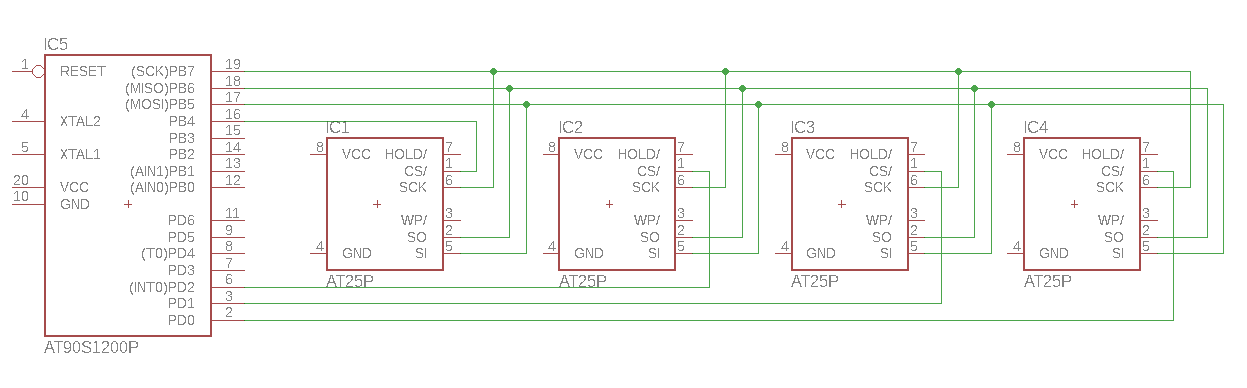
\includegraphics[width=\textwidth]{spi.png}
	
	The following shows a circuit schematic for I\textsuperscript{2}C connection (1 master, 4 slaves).
	
	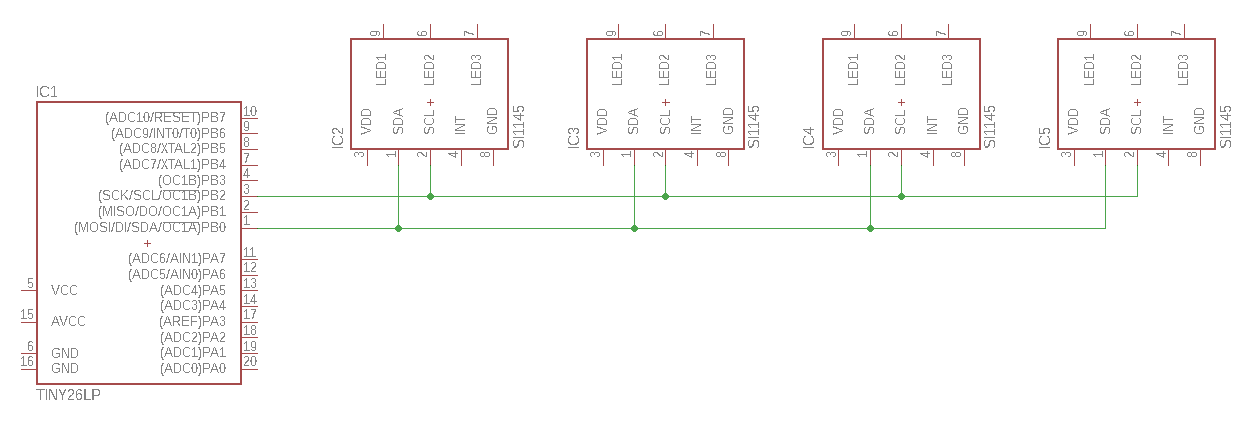
\includegraphics[width=\textwidth]{i2c.png}
	
	\item[d] The following shows exchanging the number 13 between the master and slave 2 via SPI.
	
	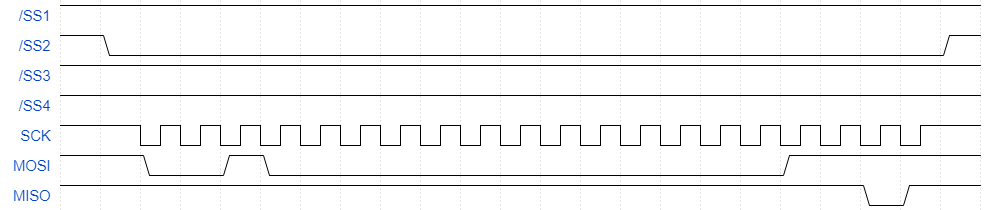
\includegraphics[width=\textwidth]{spi_wave.png}
	
	The following shows the same exchange via I\textsuperscript{2}C.
	
	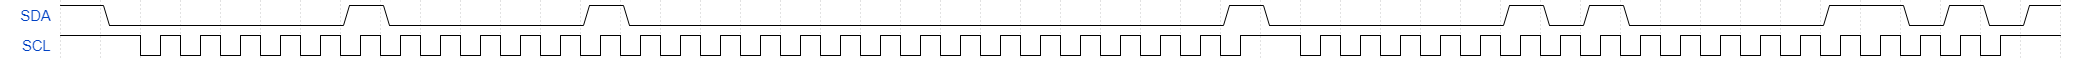
\includegraphics[width=\textwidth]{i2c_wave.png}
\end{itemize}

\end{document}
